\documentclass[conference]{IEEEtran}
\IEEEoverridecommandlockouts

\usepackage{amsmath,amssymb}
\usepackage{booktabs}
\usepackage{graphicx}
\usepackage{siunitx}
\usepackage{hyperref}
\usepackage{xcolor}

\title{Symmetry-Aware PPO for Quadrotor Hover Control:\\Interim Experimental Report}

\author{\IEEEauthorblockN{SS26 Drone Control Team}
\IEEEauthorblockA{MetaRL Project}}

\begin{document}
\maketitle

\begin{abstract}
This interim report summarizes symmetry-aware reinforcement learning experiments for quadrotor hover control. We compare baseline PPO, augmentation-only variants, mirror-loss variants, and a discretized yaw-augmentation family ($C_n$). Results are aggregated from TensorBoard logs using the mean of the final 50 \texttt{Train/mean\_reward} values per run. Augmentation-only variants provide the best performance and stability so far, while the new $C_n$ ablation indicates strongest results around $n\in\{6,8\}$.
\end{abstract}

\begin{IEEEkeywords}
quadrotor control, reinforcement learning, PPO, symmetry, data augmentation, equivariance
\end{IEEEkeywords}

\section{Introduction}
Policy learning for quadrotor control often suffers from sample inefficiency and sensitivity to nuisance transformations. Symmetry-aware RL methods improve learning by enforcing or exploiting invariances/equivariances in dynamics and observations~\cite{mukhopadhyay2020survey,sanchez2023symmetric}. In this project, we focus on yaw symmetry for hover control and evaluate practical gains in PPO training.

\section{Experimental Setup}
\subsection{Task and training}
We train PPO agents on a direct RL quadrotor hover environment with reward terms for velocity regularization and distance-to-goal tracking. The compared experiment families are:
\begin{itemize}
    \item \textbf{baselines}: standard PPO.
    \item \textbf{aug\_only}: symmetry data augmentation only.
    \item \textbf{aug\_only\_c4}: fixed $C_4$ augmentation.
    \item \textbf{mirror\_loss\_only}: mirror loss only.
    \item \textbf{aug\_plus\_mirror\_loss}: augmentation + mirror loss.
    \item \textbf{aug\_mirror}: historical combined family in logs.
\end{itemize}

\subsection{Metric aggregation}
For each run, we compute
\begin{equation}
R_{\mathrm{final}} = \frac{1}{K}\sum_{i=1}^{K} r_i, \quad K=\min(50, N_{\mathrm{logged}}),
\end{equation}
where $r_i$ are the final scalar values of \texttt{Train/mean\_reward}. We then report mean and standard deviation across runs for each family.

\section{Results}
\subsection{Family-level comparison}
\begin{table}[t]
\caption{Final reward summary by experiment family.}
\label{tab:family}
\centering
\begin{tabular}{lrrrrr}
\toprule
Family & Runs & Mean & Std & Min & Max \\
\midrule
baselines & 11 & 127.11 & 4.60 & 117.06 & 132.31 \\
aug\_only & 11 & 131.41 & 2.26 & 125.71 & 133.97 \\
aug\_only\_c4 & 11 & 131.30 & 1.59 & 127.28 & 132.66 \\
mirror\_loss\_only & 3 & 124.44 & 4.59 & 118.61 & 129.82 \\
aug\_plus\_mirror\_loss & 3 & 127.43 & 3.15 & 123.32 & 130.96 \\
aug\_mirror & 12 & 122.74 & 13.42 & 98.85 & 133.97 \\
\bottomrule
\end{tabular}
\end{table}

Augmentation-only variants outperform baseline by roughly 4.2 reward points on average and have lower variance, indicating improved optimization stability.

\subsection{$C_n$ discretization ablation}
We also evaluate a discretized yaw augmentation family under \texttt{aug\_only\_theta}, with classes $C_4$, $C_6$, $C_8$, and $C_{12}$.

\begin{table}[t]
\caption{$C_n$ ablation (3 runs/class).}
\label{tab:cn}
\centering
\begin{tabular}{lrrrrr}
\toprule
Class & Runs & Mean & Std & Min & Max \\
\midrule
$C_4$ & 3 & 130.85 & 1.05 & 129.36 & 131.65 \\
$C_6$ & 3 & 131.29 & 0.41 & 130.73 & 131.70 \\
$C_8$ & 3 & 131.28 & 1.25 & 130.02 & 132.98 \\
$C_{12}$ & 3 & 126.90 & 2.84 & 123.36 & 130.33 \\
\bottomrule
\end{tabular}
\end{table}

Current evidence suggests moderate discretization ($n=6$ or $8$) provides the best trade-off between peak reward and stability.

\begin{figure}[t]
    \centering
    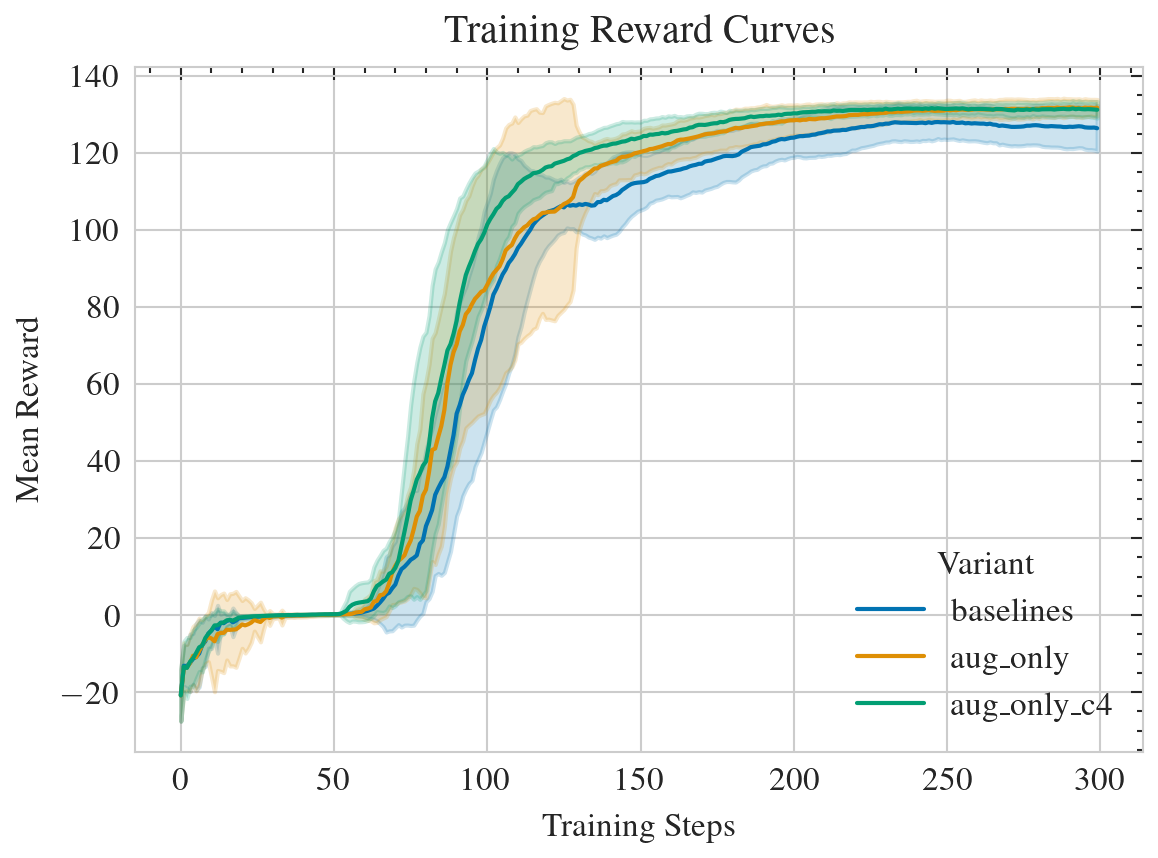
\includegraphics[width=0.98\linewidth]{figures/training_reward_curves.png}
    \caption{Training reward curves for baseline and main symmetry families.}
    \label{fig:maincurves}
\end{figure}

\begin{figure}[t]
    \centering
    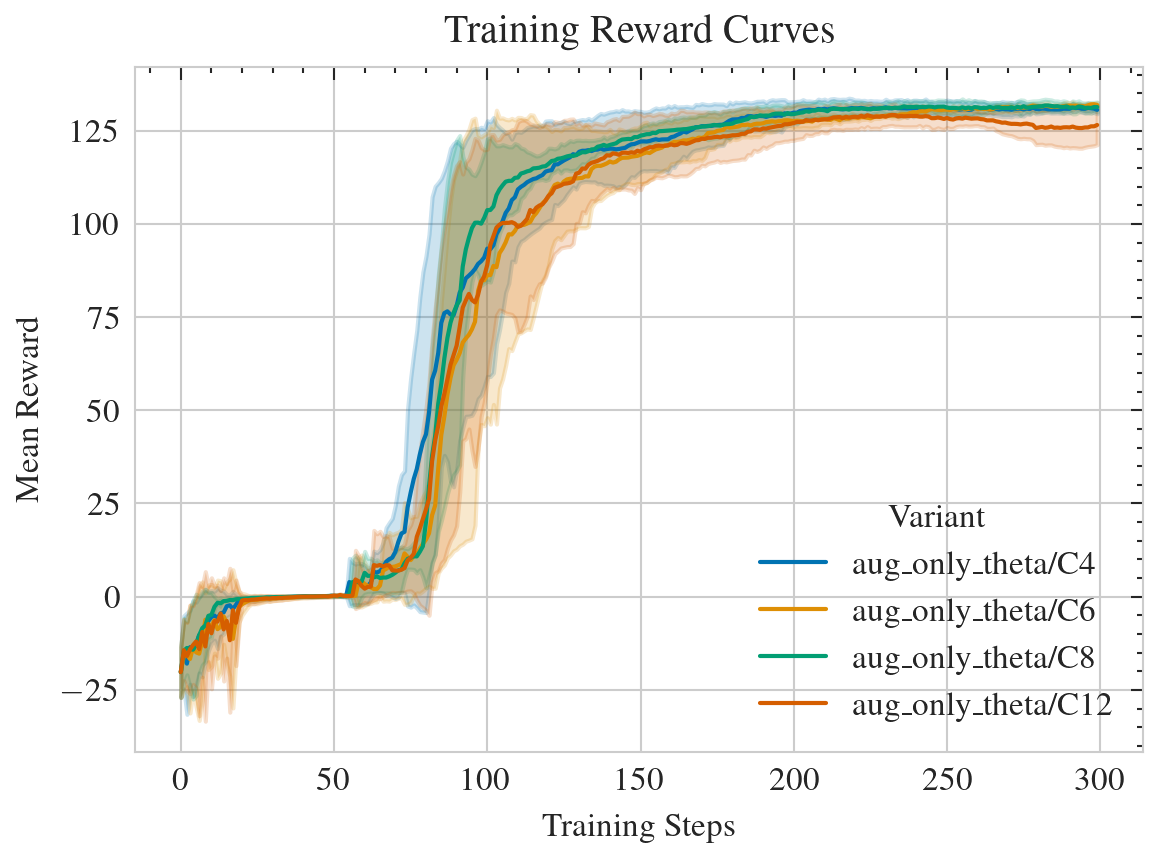
\includegraphics[width=0.98\linewidth]{figures/training_reward_curves_Cn.png}
    \caption{Training reward curves for discretized yaw classes ($C_n$).}
    \label{fig:cncurves}
\end{figure}

\section{Discussion}
The strongest trend so far is the consistent gain from augmentation-only methods over baseline PPO. Mirror-loss-only and combined mirror-loss variants underperform in current settings, suggesting either suboptimal coefficient selection or an interaction with training budget.

\section{Threats to Validity}
\begin{itemize}
    \item Several groups use only 3 seeds; uncertainty remains high.
    \item Metrics are training-time only; robustness and transfer are not yet included.
    \item Historical runs may differ in minor hyperparameter details.
\end{itemize}

\section{Next Steps}
\begin{itemize}
    \item Expand seed count for all $C_n$ variants to at least 10.
    \item Run focused sweep around $n\in\{4,6,8,10\}$ under equal budgets.
    \item Perform mirror-loss coefficient sweeps with matched augmentation settings.
    \item Add evaluation metrics: final goal error distribution and disturbance recovery.
\end{itemize}

\section*{Acknowledgment}
This manuscript is an interim lab report generated from in-repo training logs and notebook plots.

\bibliographystyle{IEEEtran}
\bibliography{references}

\end{document}
